\documentclass[a4paper]{article}
\usepackage{indentfirst}
\usepackage{setspace}
\usepackage{graphicx}
\graphicspath{{./Terms/}}
\usepackage[14pt]{extsizes}
\usepackage[utf8]{inputenc}
\usepackage[T2A]{fontenc}
\usepackage[russian]{babel}
\usepackage[left=20mm, top=20mm, right=15mm, bottom=20mm, nohead, footskip=10mm]{geometry}
\begin{document}
\thispagestyle{empty}
\begin{center}
  Министерство образования Республики Беларусь \\
\end{center}


\begin{center}
  Учреждение образования\\
  БЕЛОРУССКИЙ ГОСУДРАСТВЕННЫЙ УНИВЕРСИТЕТ \\ ИНФОРМАТИКИ И РАДИОЭЛЕКТРОНИКИ
\end{center}

\begin{center}
  Факультет информационных технологий и управления \\
  Кафедра интеллектуальных информационных технологий
\end{center}

\vspace{6em}

\begin{center}
\textbf{РАСЧЕТНАЯ РАБОТА} \\ 
по дисциплине "Традиционные и интеллектуальные информационные \\ технологии" \\
на тему \\
\textbf{Задача поиска точек сочленения в неориентированном графе}
\end{center}

\vspace{15em}


\newbox{\lbox}
\savebox{\lbox}{\hbox{В.Д.Хорошавин}}
\newlength{\maxl}
\setlength{\maxl}{\wd\lbox}
\hfill\parbox{16.5cm}
{
\hspace*{5cm}\hspace*{-5cm}Выполнил:\hfill\hbox to 4.3cm {В.Д. Хорошавин\hfill}\\\\
\hspace*{5cm}\hspace*{-5cm}Студент группы \\ 021704\\
\hspace*{5cm}\hspace*{-5cm}Проверил:\hfill\hbox to 4.3cm {В.С. Витязь\hfill}\\
}


\vspace{\fill}

\begin{center}
Минск 2021
\end{center}
\newpage
\setcounter{page}{1}
\textbf{Цель:} Получить навыки формализации и обработки информации с использованием семантических сетей \par
\textbf{Задача:} Поиск точек сочленения в неориентированном графе
\section{СПИСОК ПОНЯТИЙ}
\begin{enumerate}
  \item Графовая структура (абсолютное понятие) - это такая одноуровневая реляционная структура, объекты которой могут играть роль либо вершины, либо связки:
    \begin{enumerate}
      \item Вершина (относительное понятие, ролевое отношение);
      \item Связка (относительное понятие, ролевое отношение).
    \end{enumerate}
    \begin{figure}[h]
      \center{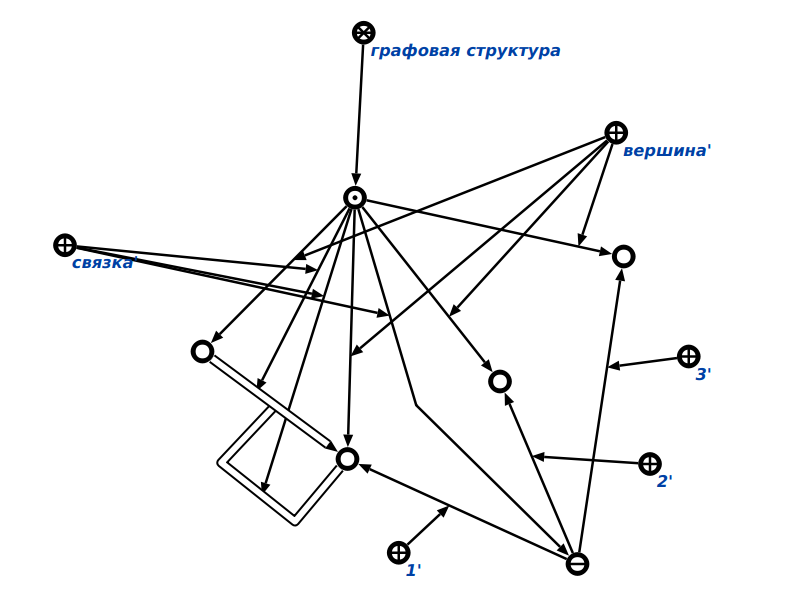
\includegraphics[scale=0.5]{Графовая структура.png}}
      \caption{Графовая структура}
    \end{figure}
  \item Графовая структура с ориентированными связками (абсолютное понятие)
    \begin{enumerate}
      \item Ориентированная связка (относительное понятие, ролевое отношение) – связка, которая задается ориентированным множеством.
    \end{enumerate}
    \begin{figure}[!ht]
      \center{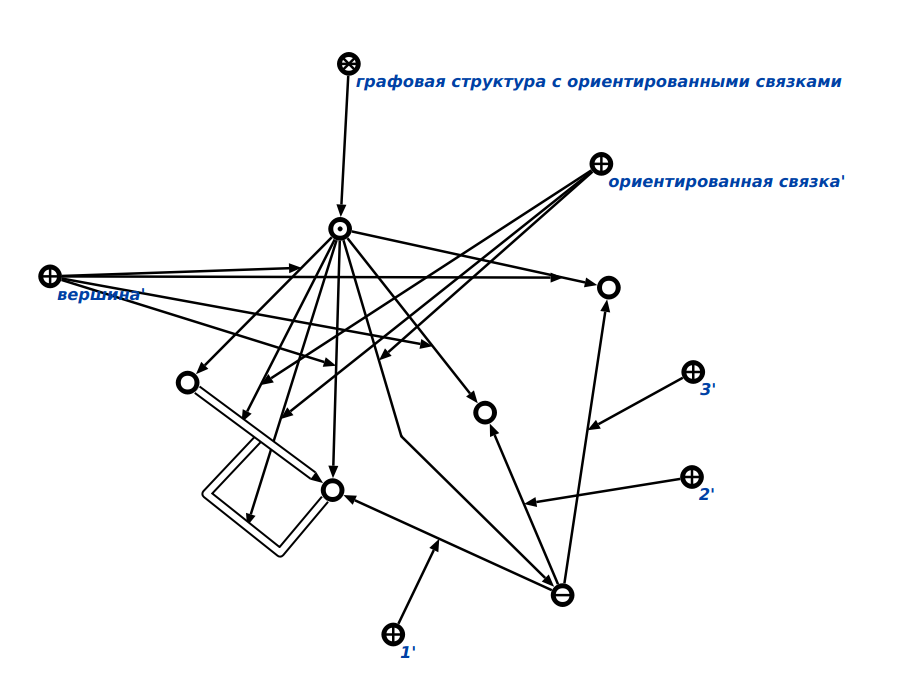
\includegraphics[scale=0.5]{Графовая структура с ориентированными связками.png}}
      \caption{Графовая структура с ориентированными связками}
    \end{figure}
\newpage
  \item Графовая структура с неориентированными связками (абсолютное понятие)
    \begin{enumerate}
      \item Неориентированная связка (относительное понятие, ролевое отношение) – связка, которая задается неориентированным множеством. 
    \end{enumerate}
    \begin{figure}[!ht]
      \center{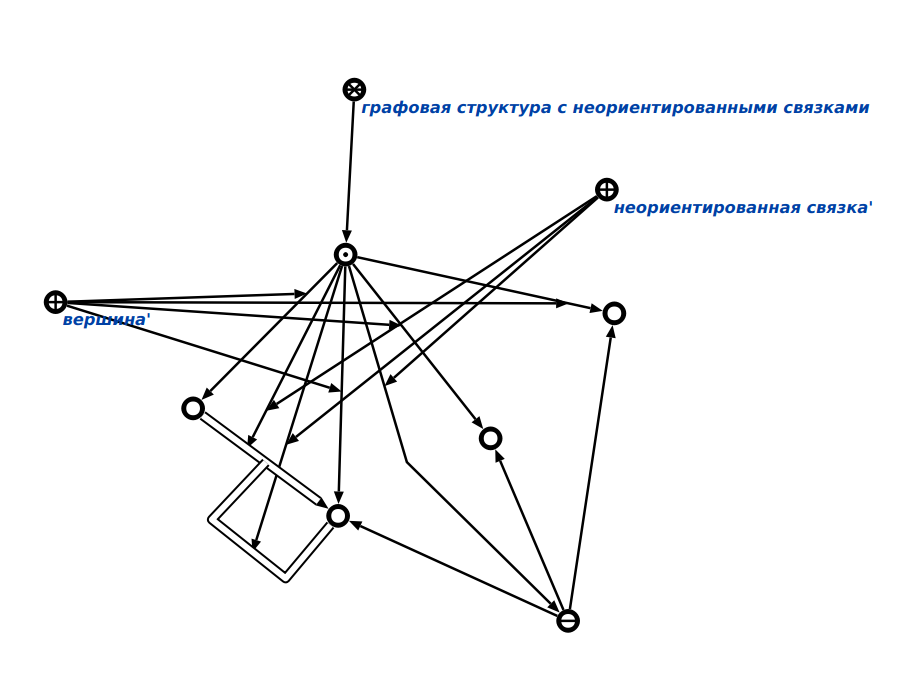
\includegraphics[scale=0.5]{Графовая структура с неориентированными связками.png}}
      \caption{Графовая структура с неориентированными связками}
    \end{figure}
\newpage
  \item Гиперграф (абсолютное понятие) – это такая графовая структура, в которой связки могут связывать только вершины:
    \begin{enumerate}
      \item Гиперсвязка (относительное понятие, ролевое отношение);
      \item Гипердуга (относительное понятие, ролевое отношение) – ориентированнаягиперсвязка;
      \item Гиперребро (относительное понятие, ролевое отношение) – неориентированная гиперсвязка.
    \end{enumerate}
    \begin{figure}[!ht]
      \center{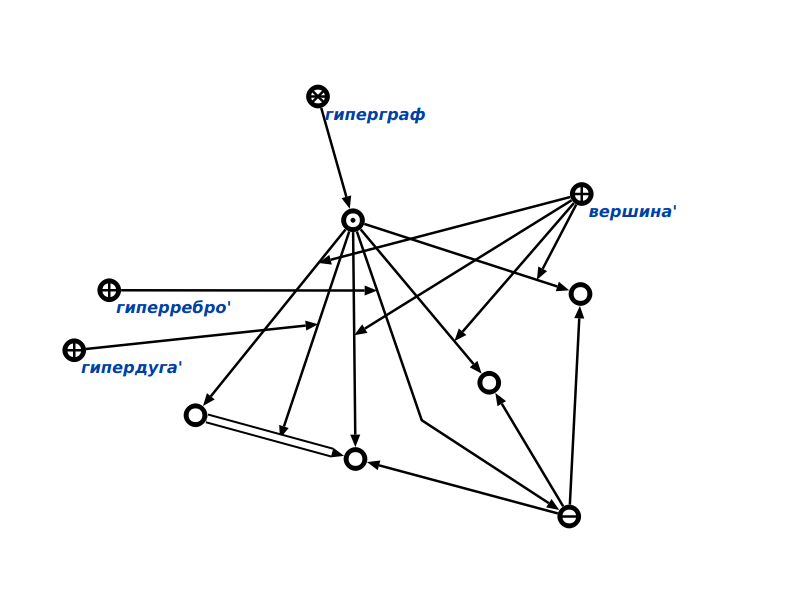
\includegraphics[scale=0.5]{Гиперграф.png}}
      \caption{Гиперграф}
    \end{figure}
\newpage
  \item Псевдограф (абсолютное понятие) – это такой гиперграф, в котором все связки должны быть бинарными:
    \begin{enumerate}
      \item Бинарная связка (относительное понятие, ролевое отношение) – гиперсвязка арности 2;
      \item Ребро (относительное понятие, ролевое отношение) – неориентированная гиперсвязка;
      \item Дуга (относительное понятие, ролевое отношение) – ориентированная гиперсвязка;
      \item Петля (относительное понятие, ролевое отношение) – бинарная связка, у которой первый и второй компоненты совпадают.
    \end{enumerate}
\newpage
    \begin{figure}[!hb]
      \center{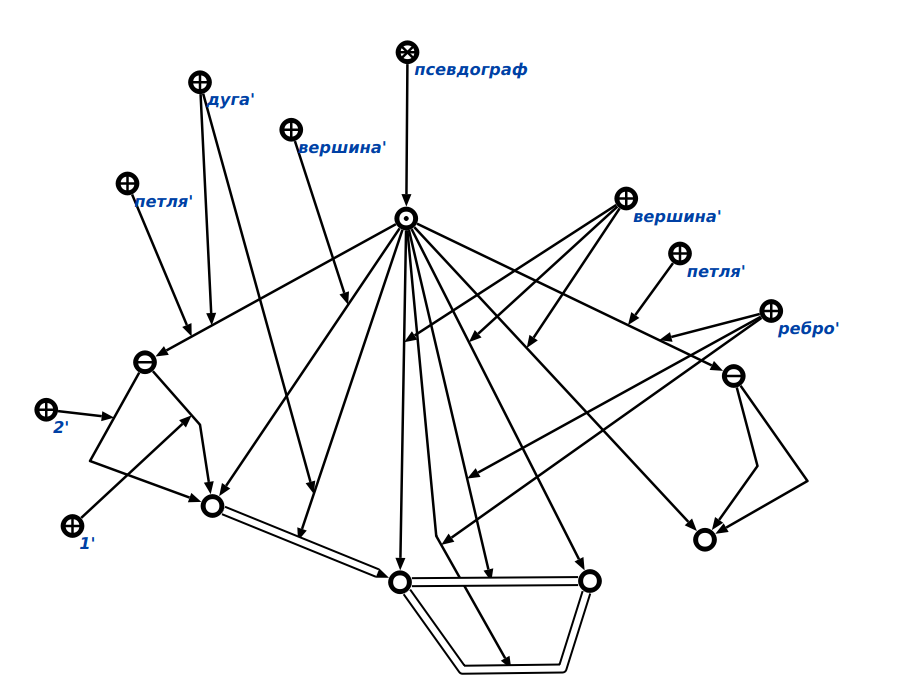
\includegraphics[scale=0.5]{Псевдограф.png}}
      \caption{Псевдограф}
    \end{figure}
  \item Мультиграф (абсолютное понятие) – это такой псевдограф, в котором не может быть петель:
    \begin{figure}[!h]
      \center{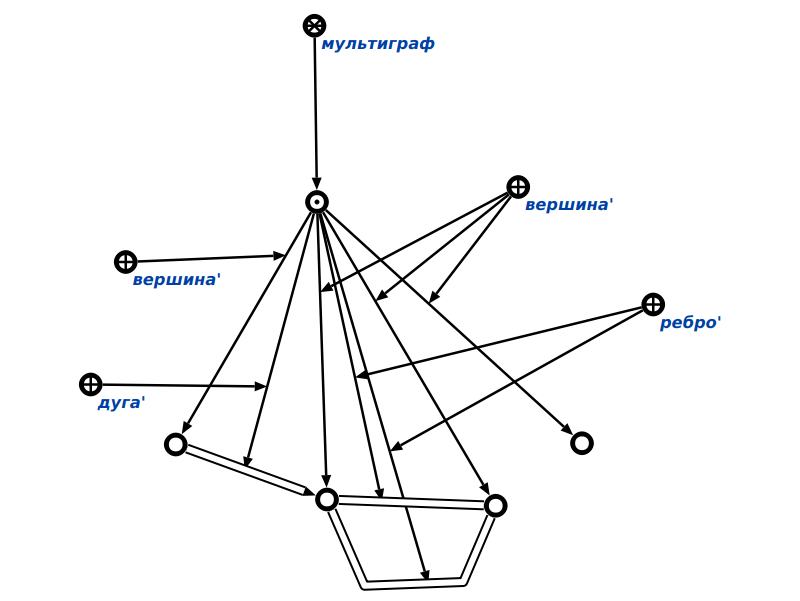
\includegraphics[scale=0.4]{Мультиграф.png}}
      \caption{Мультиграф}
    \end{figure}
  \item Граф (абсолютное понятие) – это такой мультиграф, в котором не может быть кратных связок, т.е. связок у которых первый и второй компоненты совпадают:
    \begin{figure}[!h]
      \center{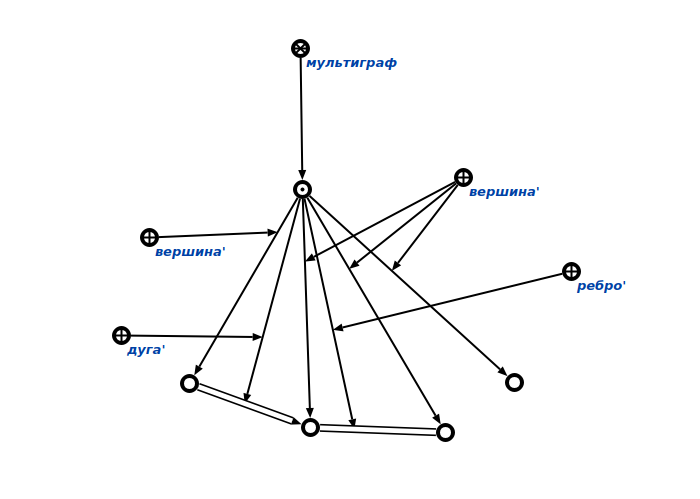
\includegraphics[scale=0.5]{Граф.png}}
      \caption{Граф}
    \end{figure}
  \item Неориентированный граф (абсолютное понятие) –это такой граф, в котором все связки являются ребрами:
    \begin{figure}[!h]
      \center{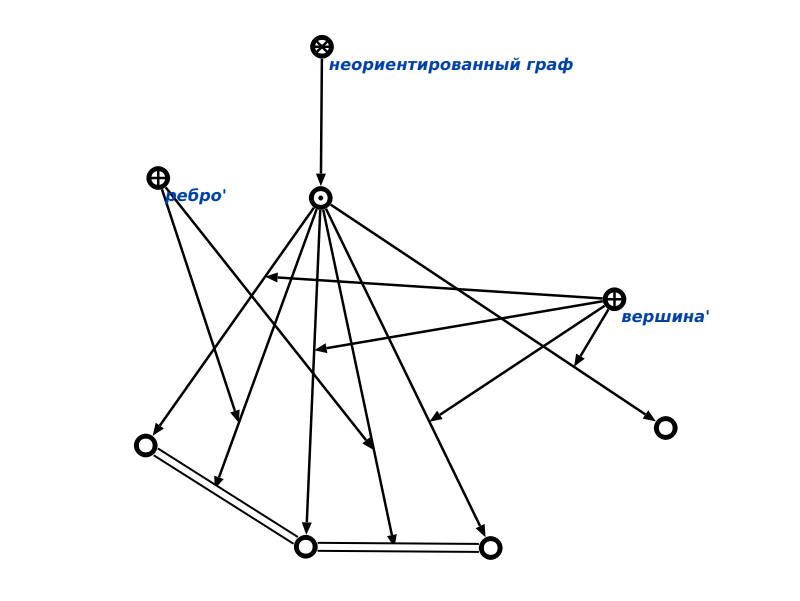
\includegraphics[scale=0.4]{Неориентированный граф.png}}
      \caption{Неориентированный граф}
    \end{figure}
  \item Связанный граф (абсолютное понятие) - граф, в котором между любой парой вершин есть путь:
    \begin{figure}[!h]
      \center{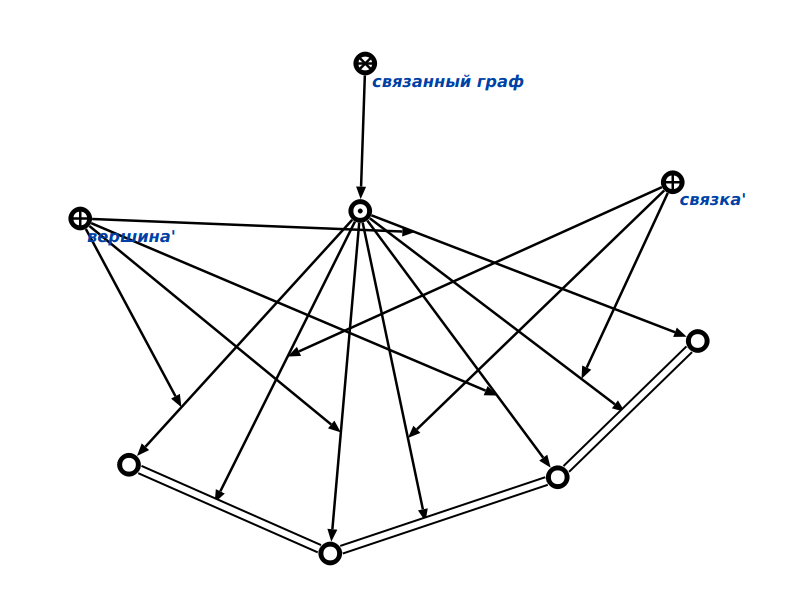
\includegraphics[scale=0.4]{Связанный граф.png}}
      \caption{Связанный граф}
    \end{figure}
  \item Точка сочленения (абсолютное понятие) - вершина при удалении которой из графа, он становится несвязанным:
    \begin{figure}[!h]
      \center{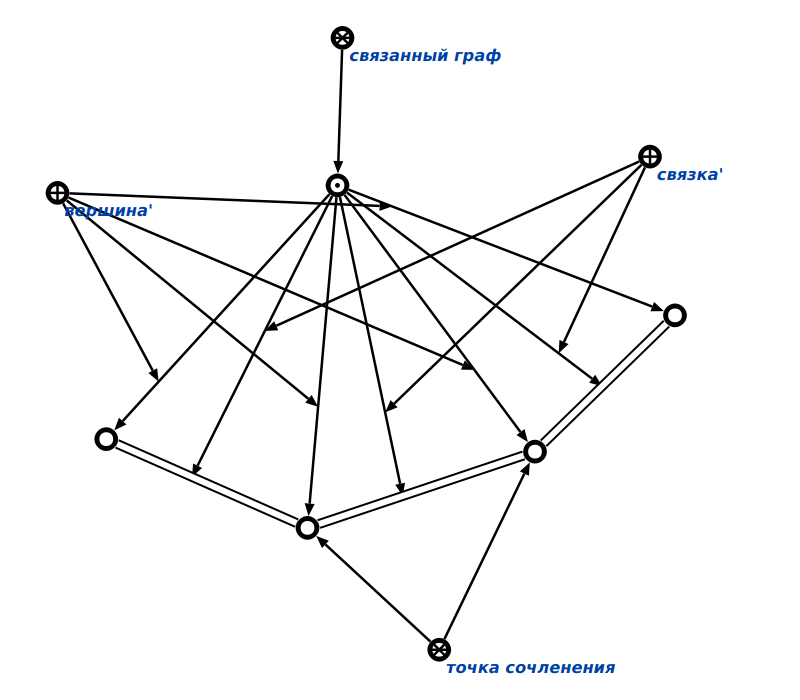
\includegraphics[scale=0.4]{Точка сочленения.png}}
      \caption{Точка сочленения}
    \end{figure}
\end{enumerate}
\newpage

\section{ТЕСТОВЫЕ ПРИМЕРЫ}

Во всех тестах графы будет приведены в сокращенной форме со скрытыми ролями элементов графа.\par
Во всех тестах решается задача поиска всех точек сочленения.

\subsection{Тест 1}

\textbf{Вход:}
  \begin{figure}[!h]
    \center{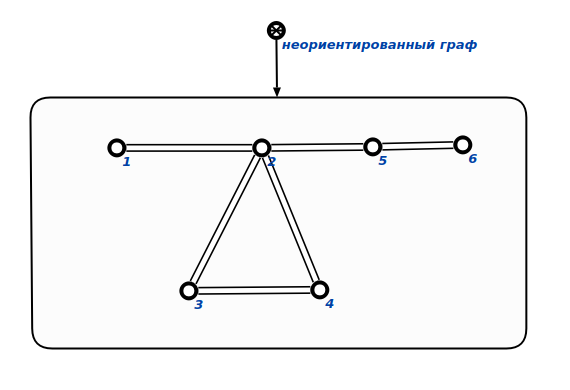
\includegraphics[scale=0.6]{./Tests/Test_1.png}}
    \caption{Вход теста 1}
  \end{figure}
\par
\textbf{Выход:} \par
  Будут найдены вершины 2 и 5:
  \begin{figure}[!h]
    \center{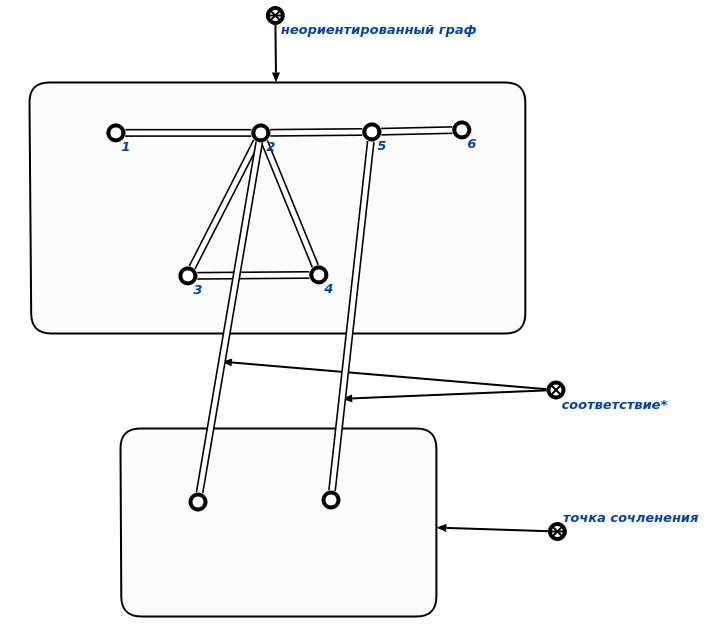
\includegraphics[scale=0.5]{./Tests/Test_1_res.png}}
    \caption{Выход теста 1}
  \end{figure}
\newpage
\subsection{Тест 2}

\textbf{Вход:}
  \begin{figure}[!h]
    \center{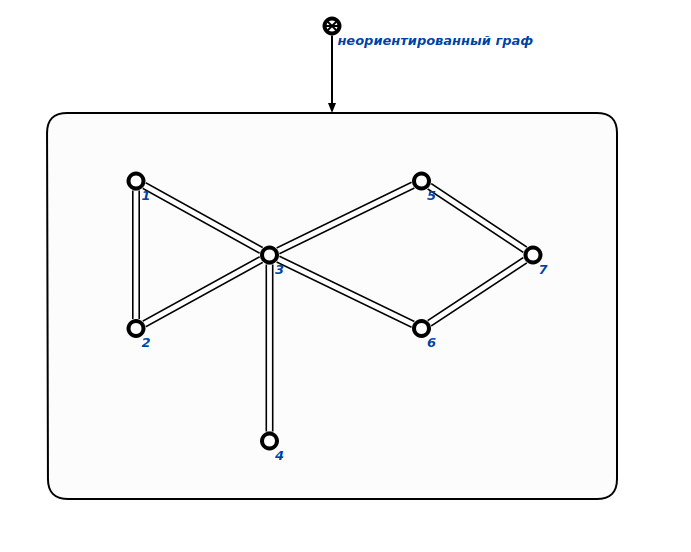
\includegraphics[scale=0.5]{./Tests/Test_2.png}}
    \caption{Вход теста 2}
  \end{figure}
\par
\textbf{Выход:} \par
  Будет найдена вершина 3:
  \begin{figure}[!h]
    \center{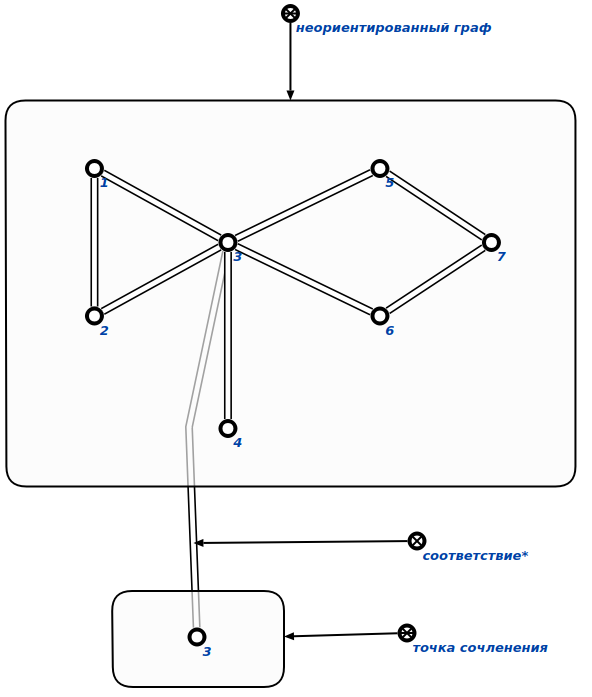
\includegraphics[scale=0.5]{./Tests/Test_2_res.png}}
    \caption{Выход теста 2}
  \end{figure}
\newpage  
\subsection{Тест 3}

\textbf{Вход:}
  \begin{figure}[!h]
    \center{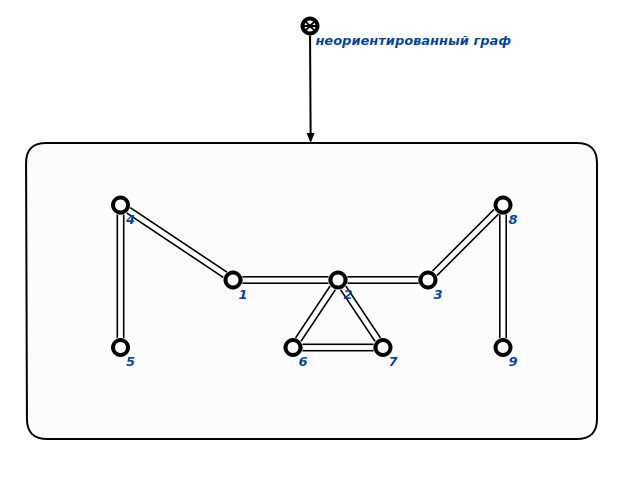
\includegraphics[scale=0.5]{./Tests/Test_3.png}}
    \caption{Вход теста 3}
  \end{figure}
\par
\textbf{Выход:} \par
  Будут найдены вершины 1, 2, 3, 4, 8:
  \begin{figure}[!h]
    \center{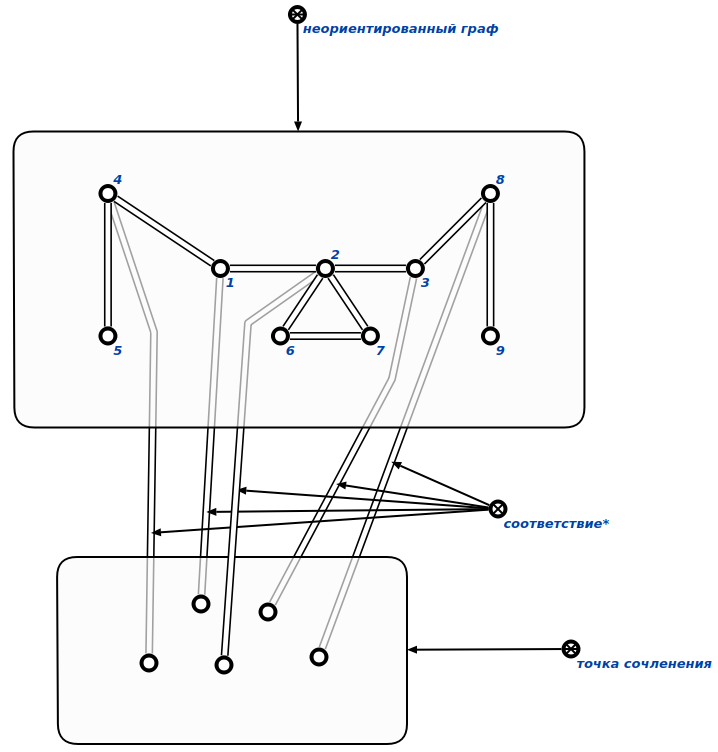
\includegraphics[scale=0.5]{./Tests/Test_3_res.png}}
    \caption{Выход теста 3}
  \end{figure}
\newpage
\subsection{Тест 4}

\textbf{Вход:}
\newpage
  \begin{figure}[!h]
    \center{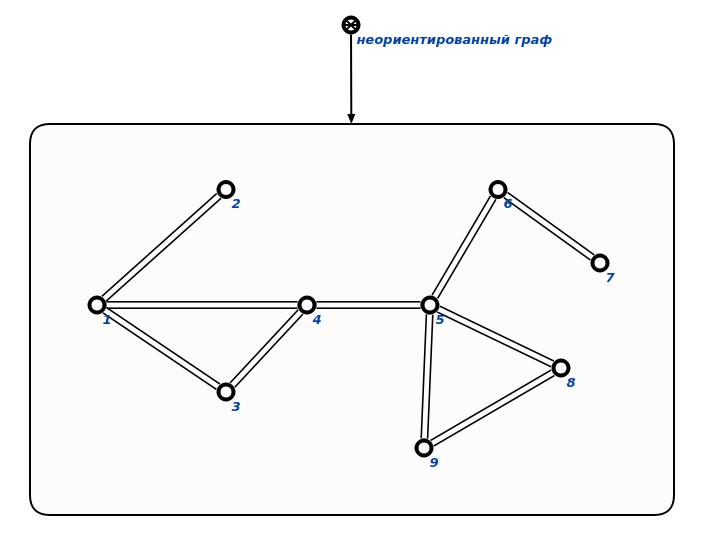
\includegraphics[scale=0.5]{./Tests/Test_4.png}}
    \caption{Вход теста 4}
  \end{figure}
\par
\textbf{Выход:} \par
  Будут найдены вершины 1, 4, 5, 6:
  \begin{figure}[!h]
    \center{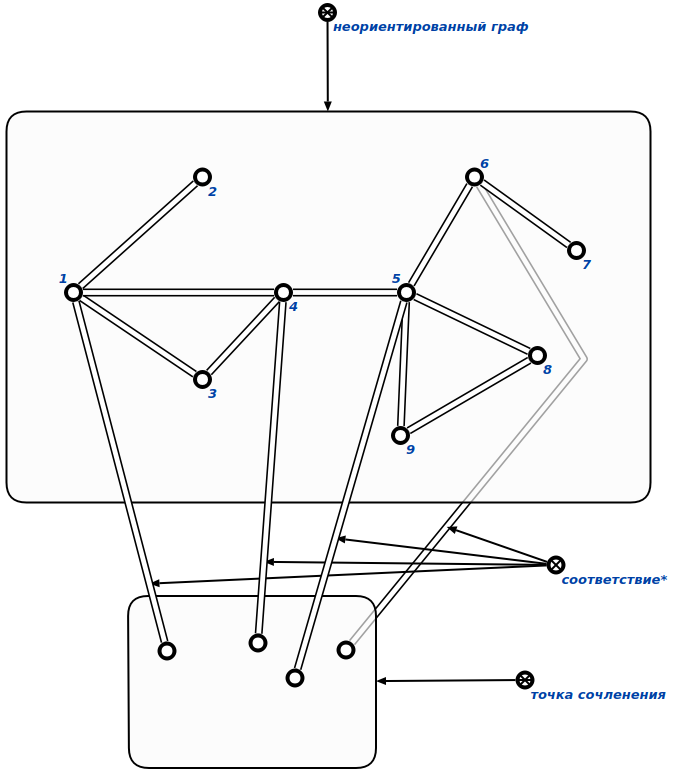
\includegraphics[scale=0.5]{./Tests/Test_4_res.png}}
    \caption{Выход теста 4}
  \end{figure}
\newpage
\subsection{Тест 5}

\textbf{Вход:}
\newpage
  \begin{figure}[!h]
    \center{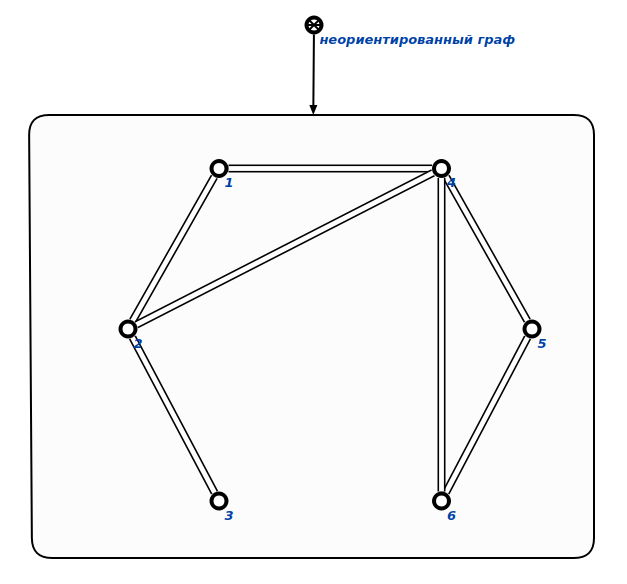
\includegraphics[scale=0.5]{./Tests/Test_5.png}}
    \caption{Вход теста 5}
  \end{figure}
\par
\textbf{Выход:} \par
  Будут найдены вершины 2, 4:
\newpage
  \begin{figure}[!h]
    \center{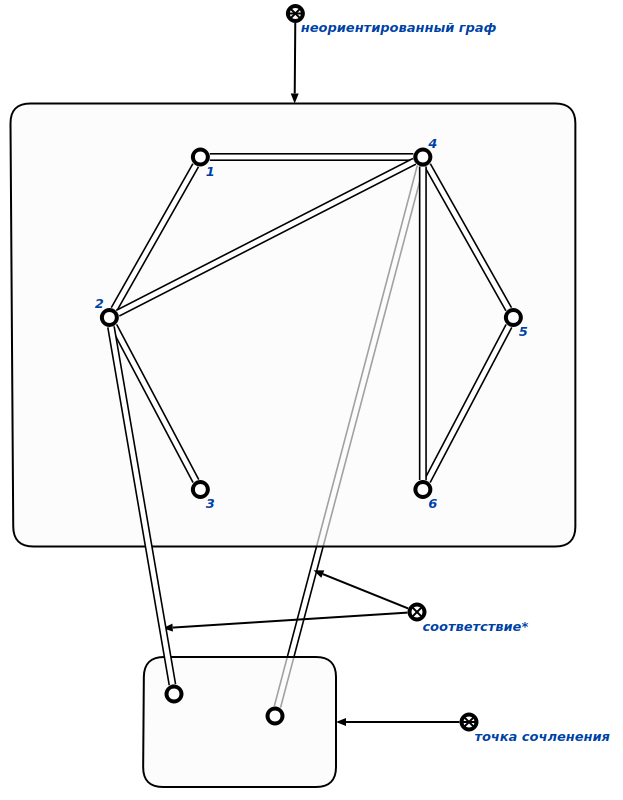
\includegraphics[scale=0.5]{./Tests/Test_5_res.png}}
    \caption{Выход теста 5}
  \end{figure}
\newpage


\onehalfspacing
\section{ПРИМЕР РАБОТЫ АЛГОРИТМА В СЕМАНТИЧЕСКОЙ ПАМЯТИ}

\textbf{Создание графа с начальными переменными (Шаг 1)}
  \begin{figure}[!h]
    \center{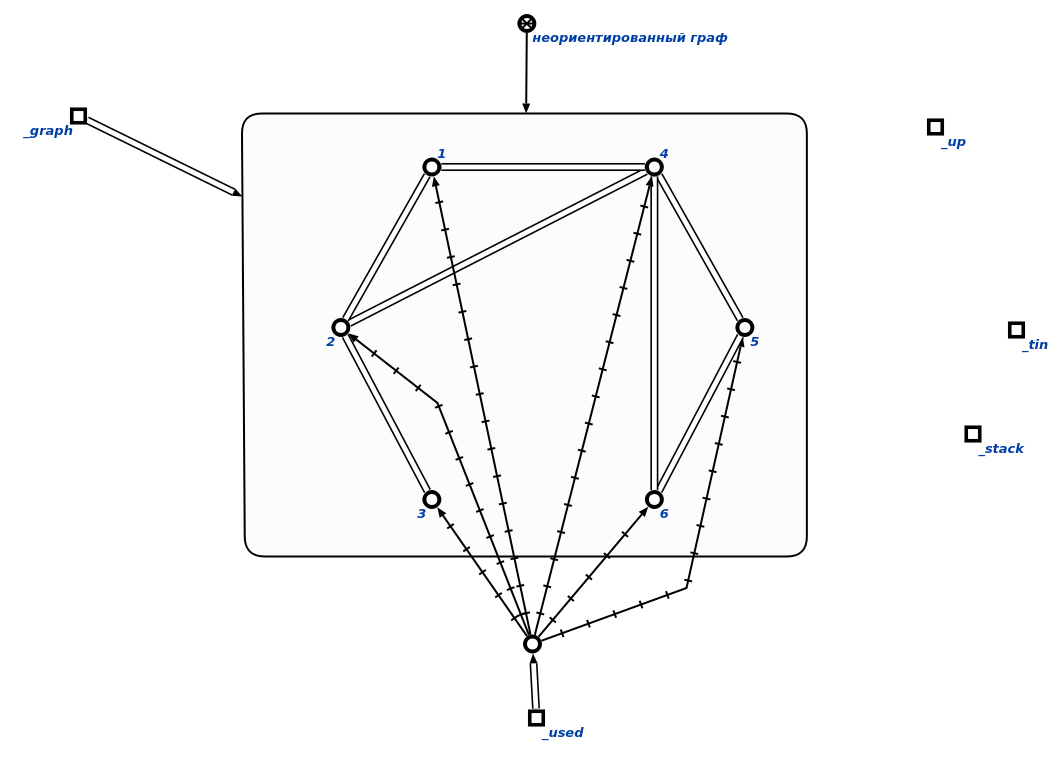
\includegraphics[scale=0.5]{./Algorythm/Step_1.png}}
  \end{figure}
\par
  \_graph получит в качестве значения sc-узел неориентированного графа\par
  \_used - множество, не содержащее элементов
\newpage
  
\textbf{Начинаем поиск в глубину из вершины 1 (Шаг 2)}
  \begin{figure}[!h]
    \center{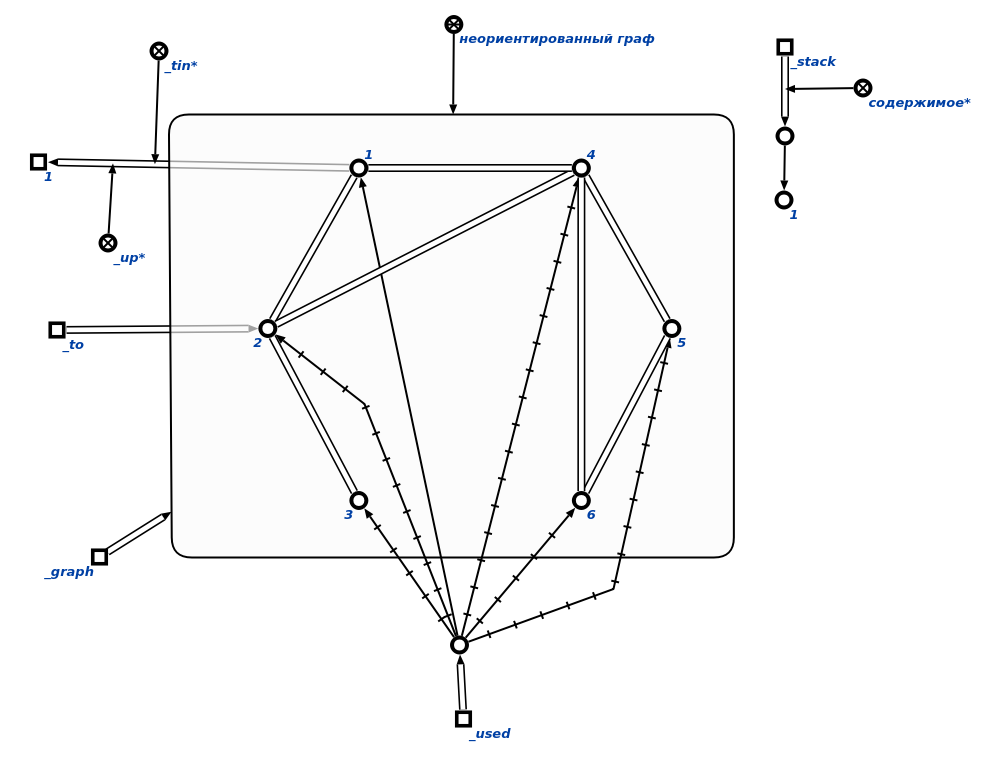
\includegraphics[scale=0.5]{./Algorythm/Step_2.png}}
  \end{figure}
\par
  В \_used добавляем вершину 1\par
  \_tin - время входа поиска в глубину в некоторую вершину\par
  \_up - время выхода поиска в глубину из некоторой вершины\par
  \_to - вершина, в которую двигается поиск в глубину\par
  \_stack - список вершин, просмотренных поиском в глубину для какой-либо вершины\par
  В \_stack добавляем вершину 1
\newpage
  
\textbf{Начинаем поиск в глубину из вершины 2 (Шаг 3)}
  \begin{figure}[!h]
    \center{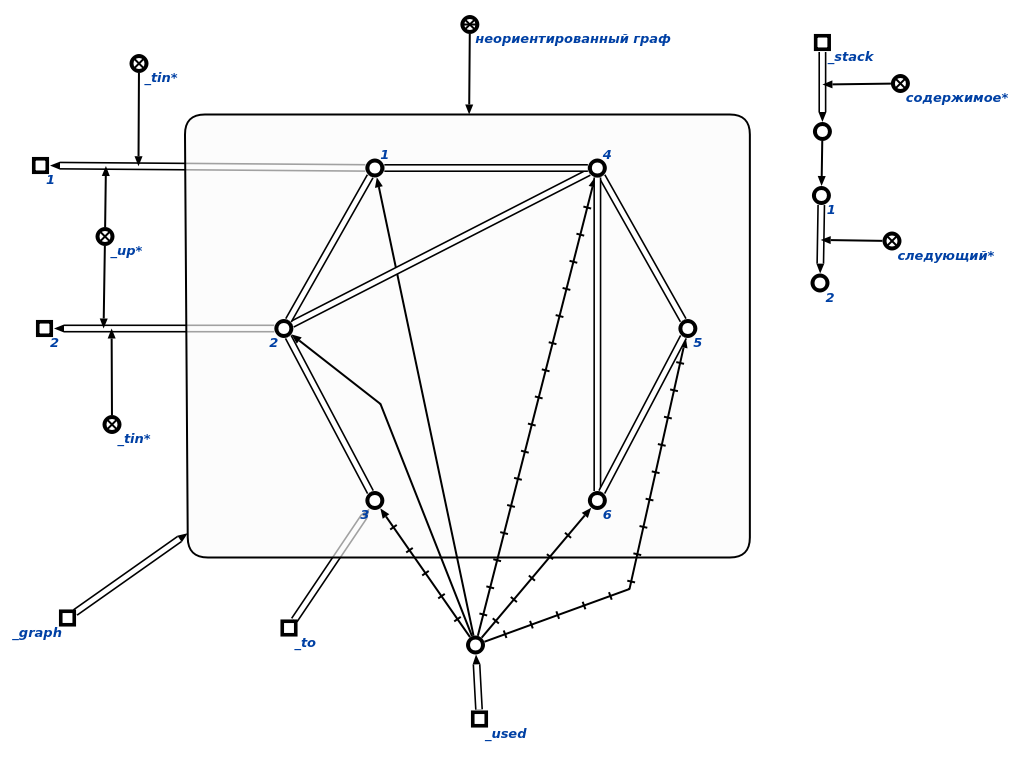
\includegraphics[scale=0.5]{./Algorythm/Step_3.png}}
  \end{figure}
\par
  В \_used добавляем вершину 2\par
  \_to получает вершину 3\par
  В \_stack добавляем вершину 2
\newpage

\textbf{Начинаем поиск в глубину из вершины 3 (Шаг 4)}
  \begin{figure}[!h]
    \center{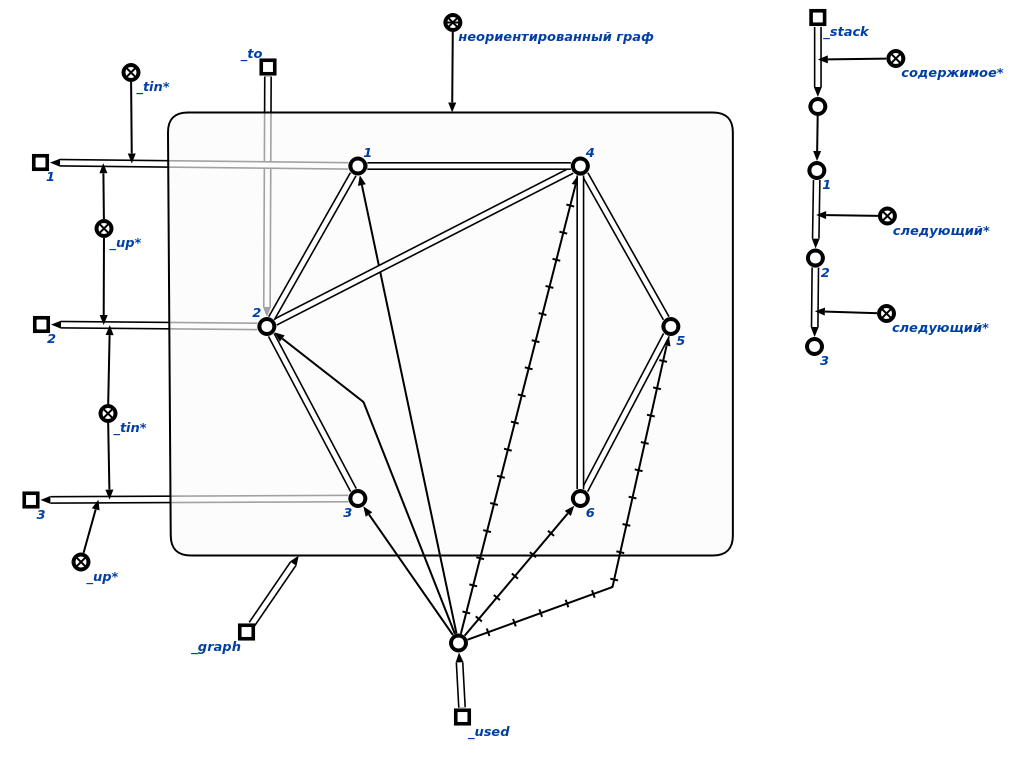
\includegraphics[scale=0.5]{./Algorythm/Step_4.png}}
  \end{figure}
\par
  В \_used добавляем вершину 3\par
  \_to получает вершину 2\par
  В \_stack добавляем вершину 3\par
  Поскольку вершина 2 уже была просмотрена и вершина 3 не имеет других смежных вершин, пересчитываем время выхода из неё.\par
  Т.к. выход из вершины 3 произошёл после входа в вершину 2, то вершина 2 является точкой сочленения.
\newpage

\textbf{Добавляем вершину 2 в множество точек сочленения (Шаг 5)}
  \begin{figure}[!h]
    \center{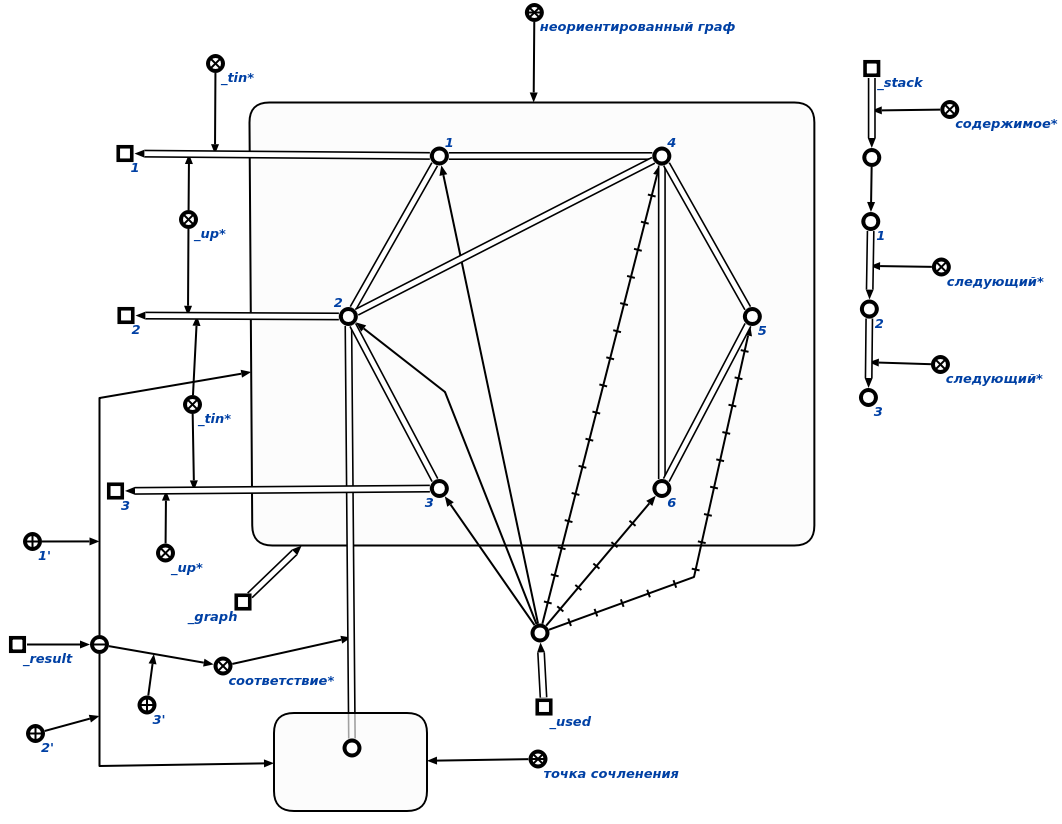
\includegraphics[scale=0.5]{./Algorythm/Step_5.png}}
  \end{figure}
\par
  Создаём переменную \_result, которая в качестве значения получит безымянную связку
\newpage

\textbf{Возвращаемся к вершине 2 и начинаем поиск в глубину из вершины 4 (Шаг 6)}
  \begin{figure}[!h]
    \center{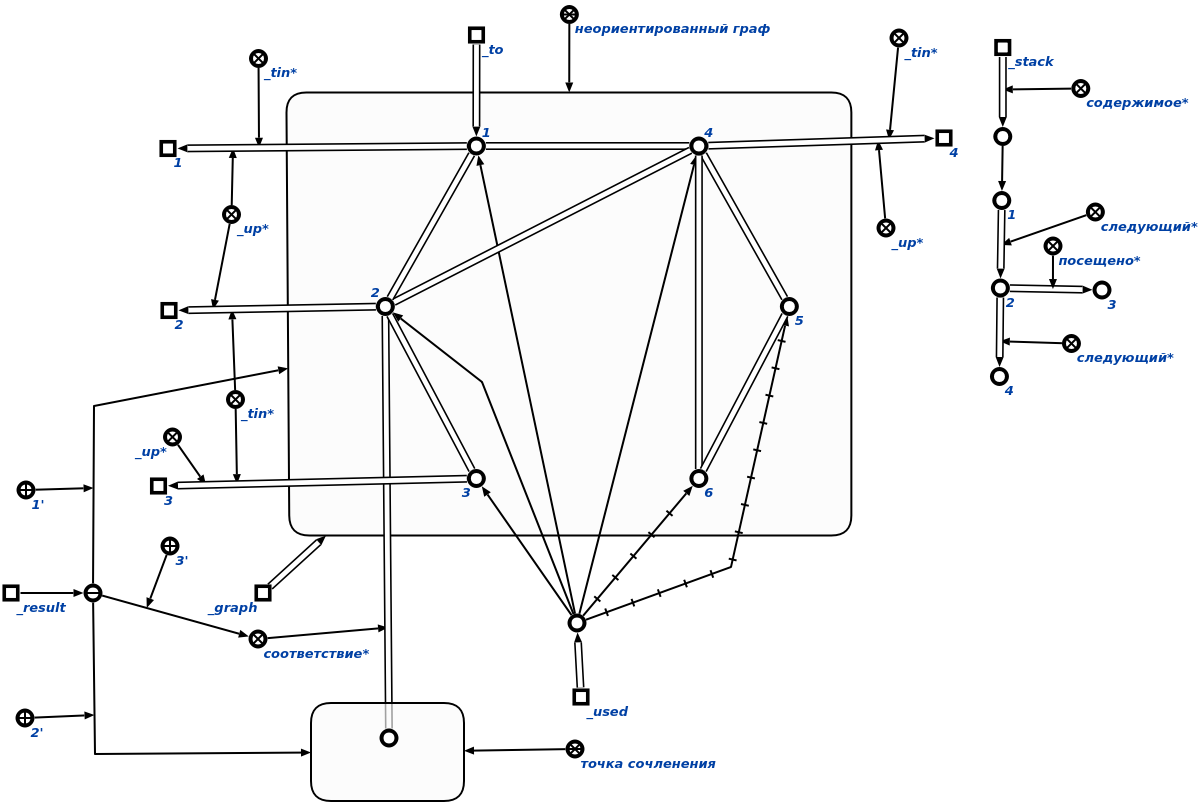
\includegraphics[scale=0.43]{./Algorythm/Step_6.png}}
  \end{figure}
\par
  В \_stack переопределяем отношение между вершинами 2 и 3 (\textit{следующий*} заменяем на \textit{посещено*})\par
  Добавляем вершину 4 в \_stack\par
  В \_used добавляем вершину 4\par
  \_to получает вершину 1\par
\newpage

  \begin{figure}[!h]
    \center{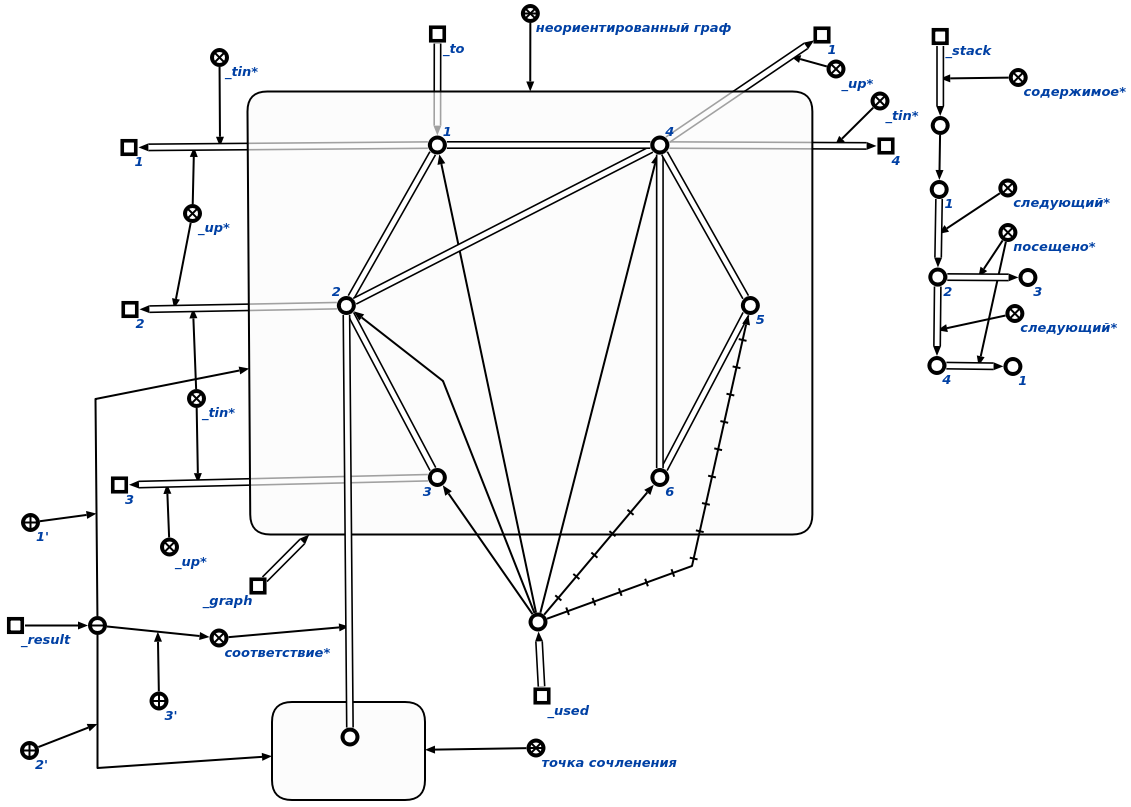
\includegraphics[scale=0.43]{./Algorythm/Step_6,1.png}}
  \end{figure}
\par
  Поскольку вершина 1 уже была просмотрена, то пересчитываем время выхода из вершины 4\par
  Отмечаем вершину 1 просмотренной при поиске в глубину из вершины 4
\newpage

\textbf{Начинаем поиск в глубину из вершины 5 (Шаг 7)}
  \begin{figure}[!h]
    \center{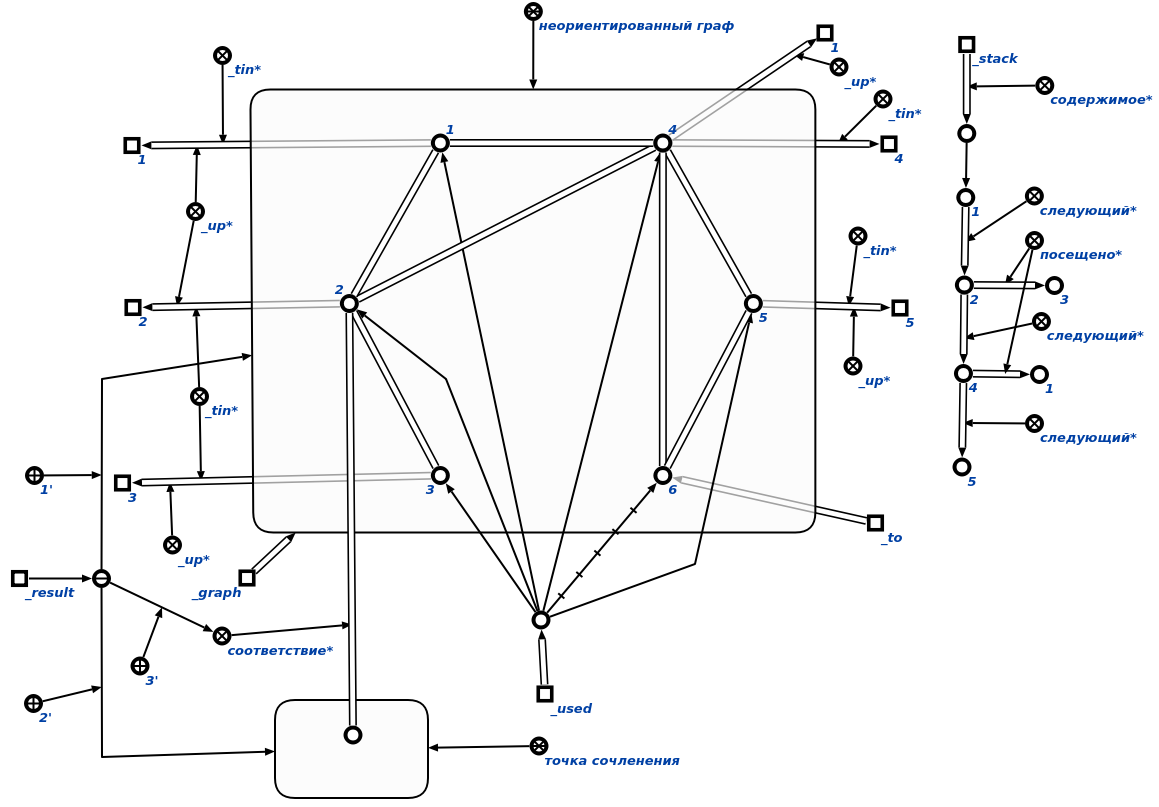
\includegraphics[scale=0.43]{./Algorythm/Step_7.png}}
  \end{figure}
\par
  Добавляем вершину 5 в \_stack\par
  В \_used добавляем вершину 5\par
  \_to получает вершину 6\par
\newpage

\textbf{Начинаем поиск в глубину из вершины 6 (Шаг 8)}
  \begin{figure}[!h]
    \center{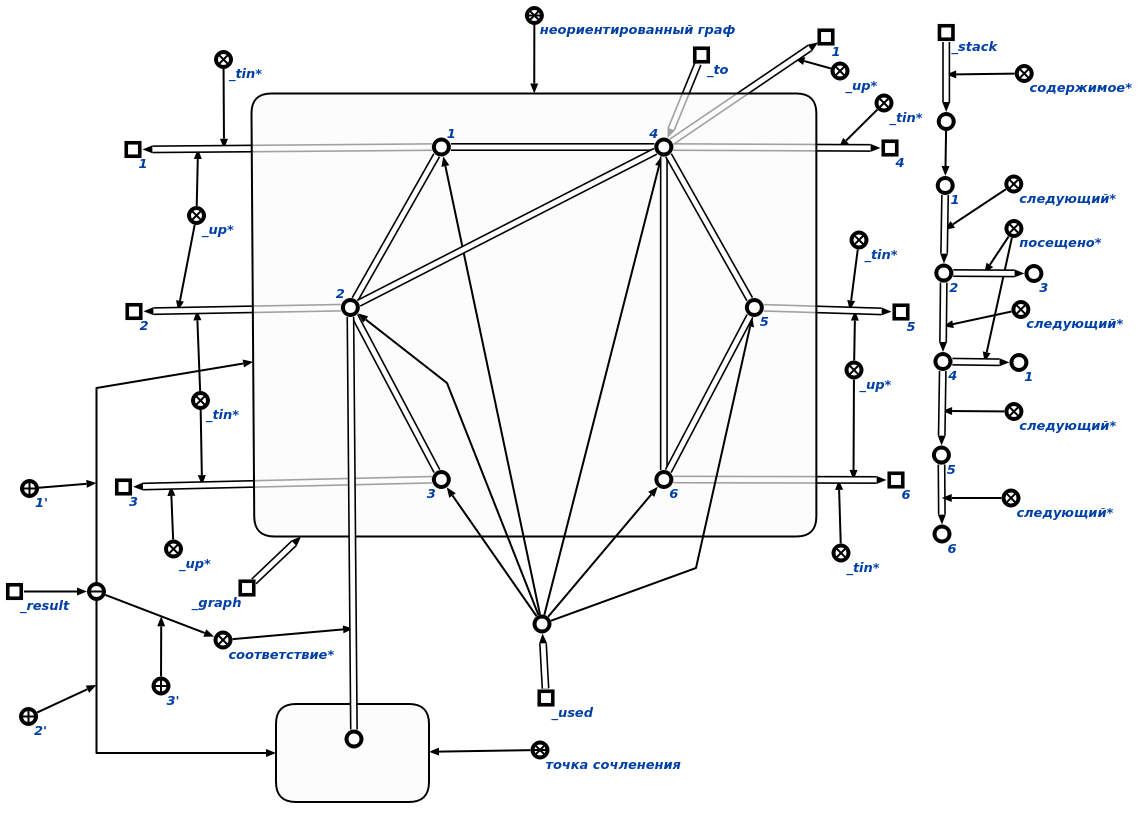
\includegraphics[scale=0.43]{./Algorythm/Step_8.png}}
  \end{figure}
\par
  В \_stack добавляем вершину 6\par
  В \_used добавляем вершину 6\par
  \_to получает вершину 4\par
\newpage

  \begin{figure}[!h]
    \center{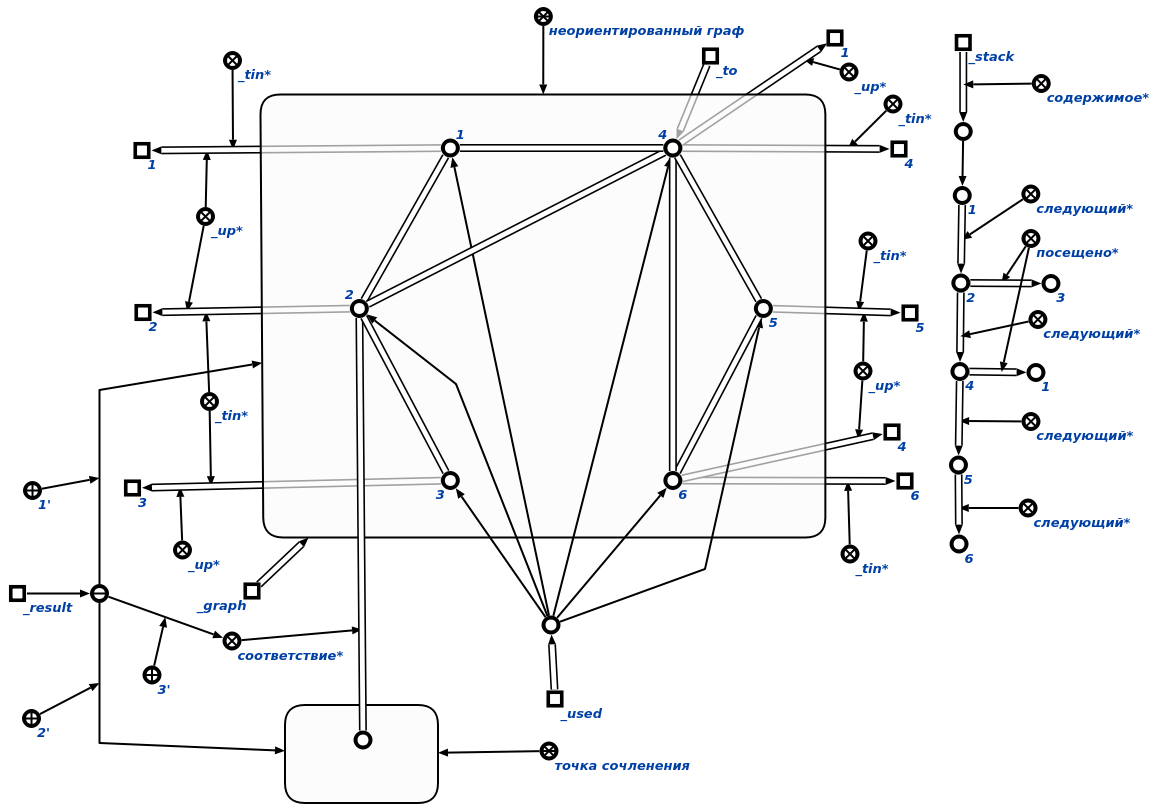
\includegraphics[scale=0.43]{./Algorythm/Step_8,1.png}}
  \end{figure}
\par
  Поскольку вершина 4 уже была просмотрена, то пересчитываем время выхода из вершины 6\par
\newpage

\textbf{Возвращаемся к вершине 5 (Шаг 9)}
  \begin{figure}[!h]
    \center{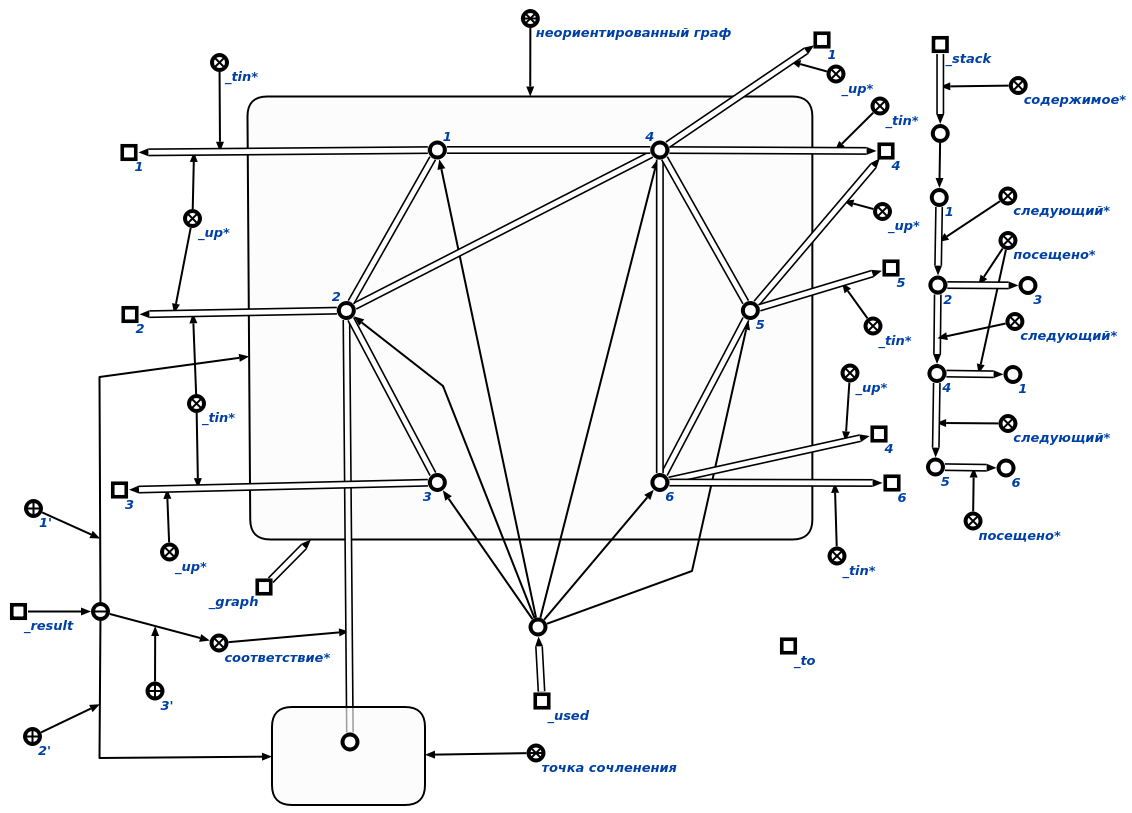
\includegraphics[scale=0.43]{./Algorythm/Step_9.png}}
  \end{figure}
\par
  Поскольку все вершины смежные с вершиной 6 уже просмотрены, пересчитываем время выхода из вершины 5\par
  Т.к. выход из вершины 6 произошёл раньше входа в вершину 5, вершина 5 не является точкой сочленения\par
  Т.к. выход из вершины 5 произошёл одновременно с входом в вершину 4, вершина 4 является точкой сочленения\par
  В \_stack переопределяем отношение между вершинами 5 и 6 (\textit{следующий*} заменяем на \textit{посещено*})
\newpage

\textbf{Добавляем вершину 4 в множество точек сочленения (Шаг 10)}
  \begin{figure}[!h]
    \center{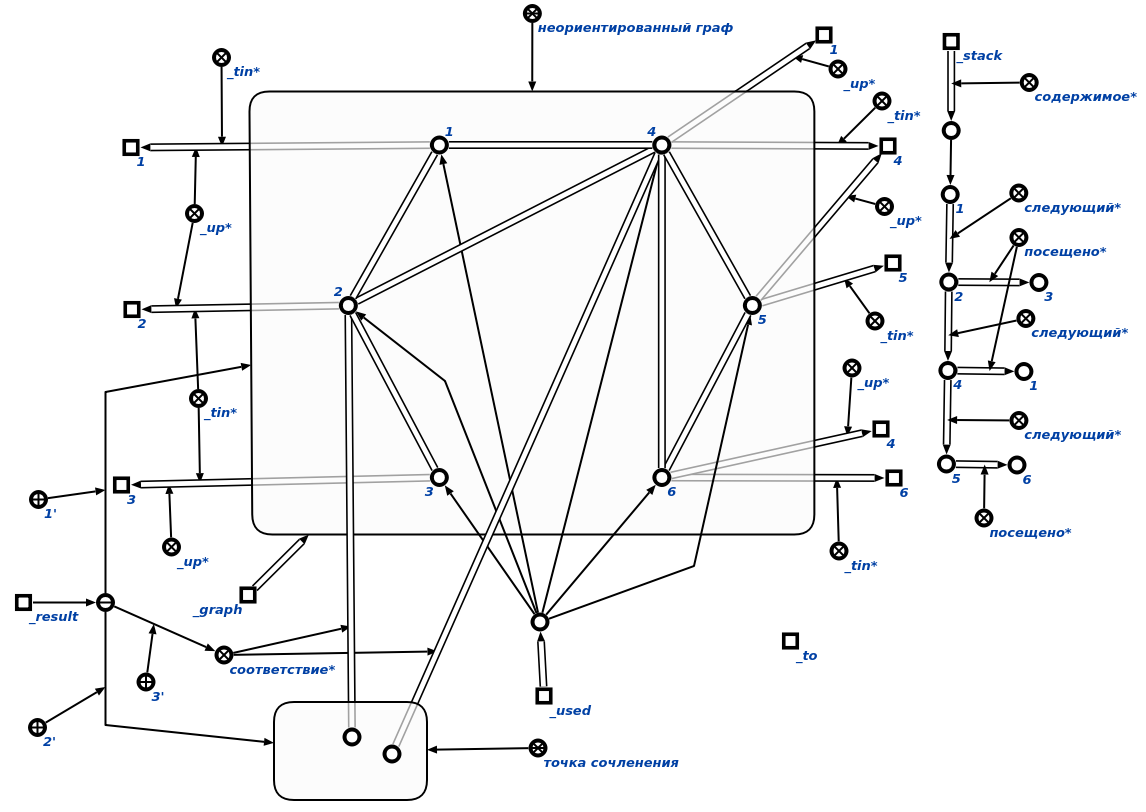
\includegraphics[scale=0.43]{./Algorythm/Step_10.png}}
  \end{figure}
\newpage

\textbf{Возвращаемся к вершине 4 (Шаг 11)}
  \begin{figure}[!h]
    \center{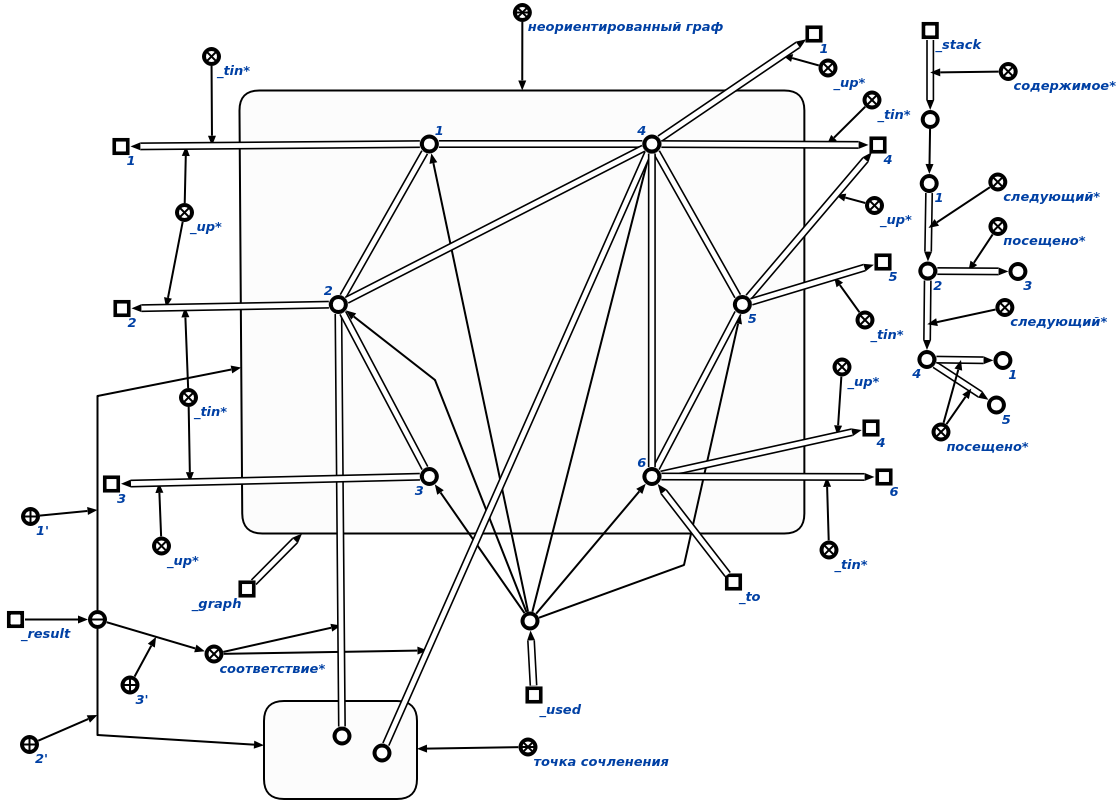
\includegraphics[scale=0.43]{./Algorythm/Step_11.png}}
  \end{figure}
\par
  В \_stack переопределяем отношение между вершинами 4 и 5 (\textit{следующий*} заменяем на \textit{посещено*})\par
  Поскольку вершина 6 уже была просмотрена, пересчитываем время выхода из вершины 4\par
  Т.к.
\newpage

\textbf{Возвращаемся к вершине 2 (Шаг 12)}
  \begin{figure}[!h]
    \center{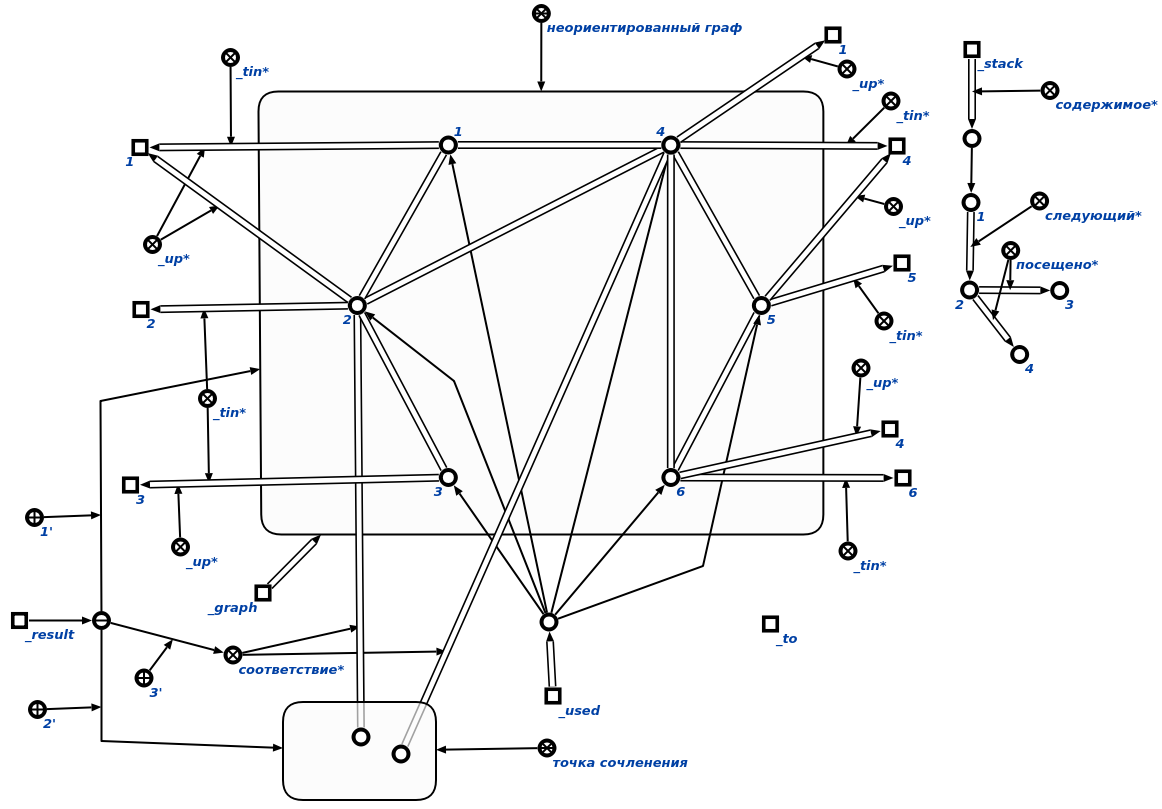
\includegraphics[scale=0.43]{./Algorythm/Step_12.png}}
  \end{figure}
\par
  В \_stack переопределяем отношение между вершинами 2 и 4 (\textit{следующий*} заменяем на \textit{посещено*})\par
  Поскольку все вершины смежные с вершиной 2 уже просмотрены, пересчитываем время выхода из вершины 2\par
\newpage

\textbf{Возвращаемся к вершине 1 (Шаг 13)}
  \begin{figure}[!h]
    \center{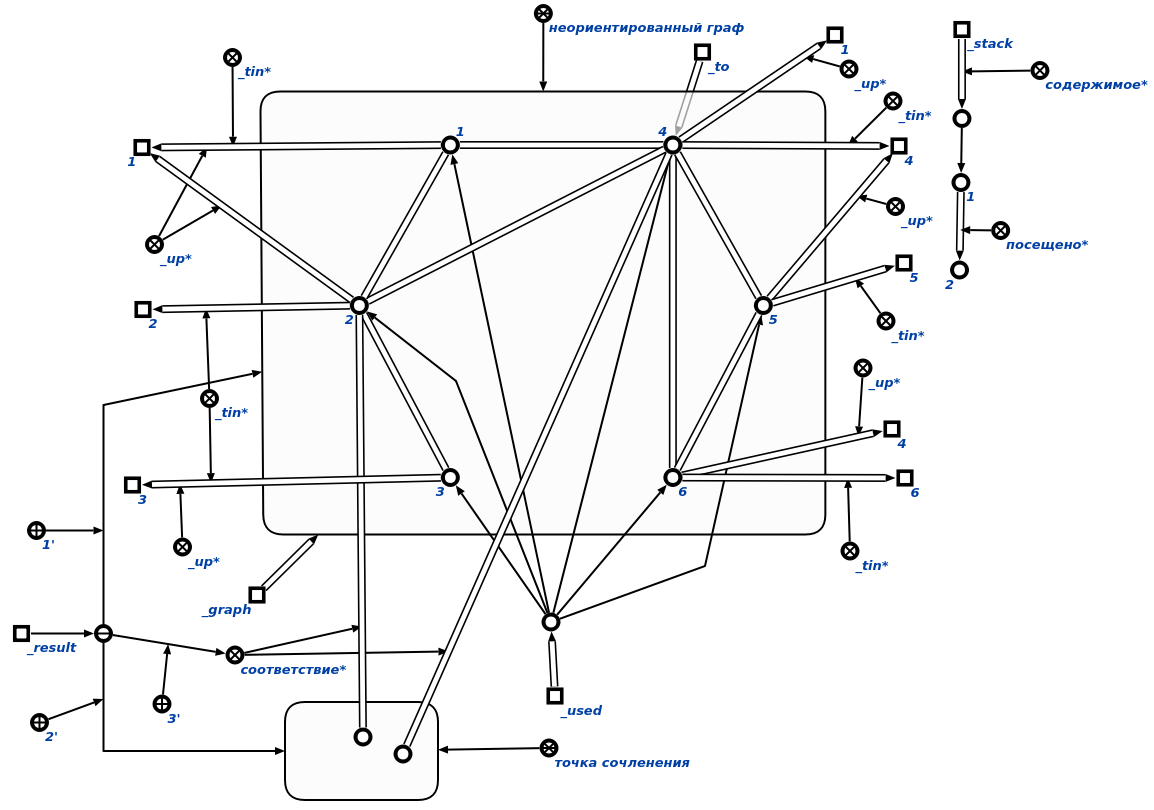
\includegraphics[scale=0.43]{./Algorythm/Step_13.png}}
  \end{figure}
\par
  Поскольку вершина 4 уже была просмотрена, пересчитываем время выхода из вершины 1\par
\newpage

\textbf{Удаление ненужных связей (Шаг 14)}
  \begin{figure}[!h]
    \center{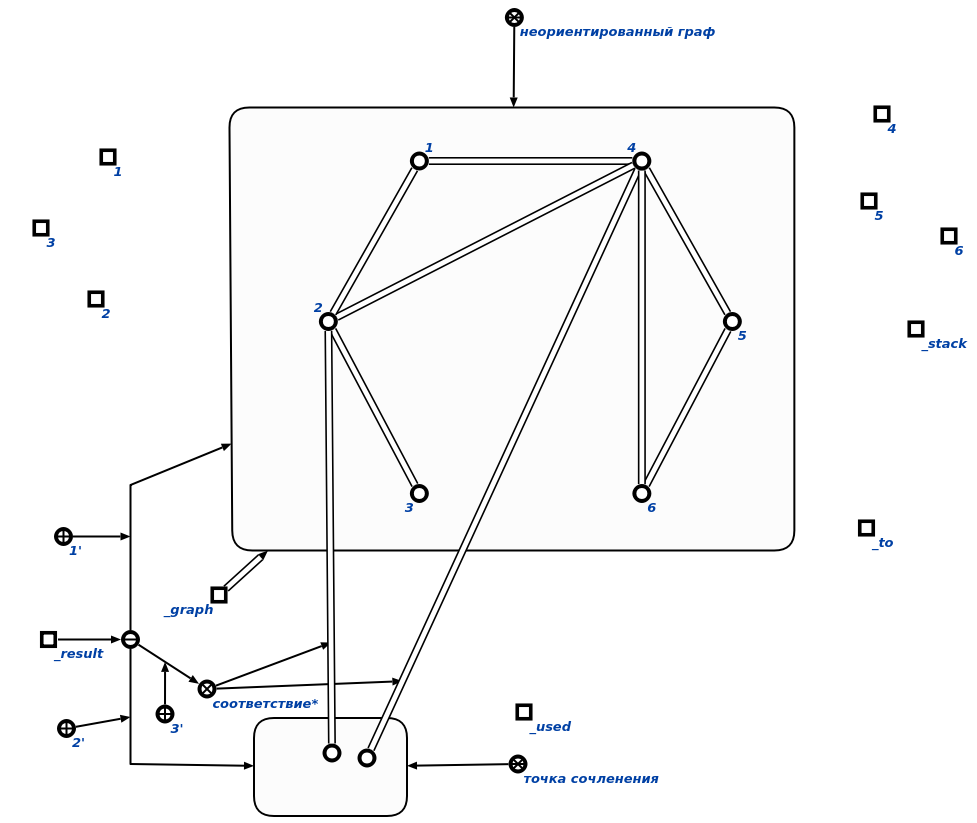
\includegraphics[scale=0.43]{./Algorythm/Step_14.png}}
  \end{figure}
\newpage

\textbf{Результат работы алгоритма}
  \begin{figure}[!h]
    \center{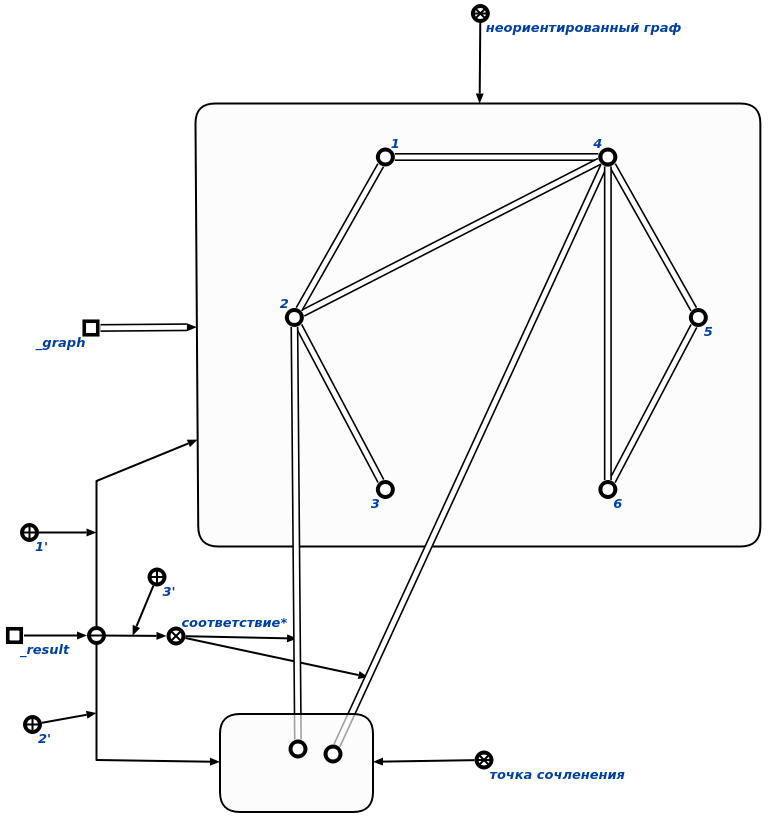
\includegraphics[scale=0.5]{./Algorythm/result.png}}
  \end{figure}
\par
  На данном этапе продемонстрирован результат работы алгоритма, значение переменной \_result будет возвращено в вызывающий контекст. 
\newpage


\section*{СПИСОК ИСПОЛЬЗОВАННЫХ ИСТОЧНИКОВ}
  [1] Кормен, Д. Алгоритмы. Построение и анализ / Д. Кормен. — Вильямс, 2015.~— P. 1328.\par
  [2] Кузнецов, О. П. Дискретная математика для инженера / О. П. Кузнецов, Г. М. Адельсон-Вельский. — Энергоатомиздат, 1988.~— P. 480.\par
  [3] Оре, О. Теория графов / О. Оре. — Наука, 1980. — P. 336.\par
  [4] Харарри, Ф. Теория графов / Ф. Харарри. — Эдиториал УРСС, 2018.~— P.~304.
\end{document}
